\documentclass{beamer}
\usepackage[utf8]{inputenc}

\setbeamertemplate{frametitle}[default][center]
\usetheme{Madrid}
\usecolortheme{default}

%------------------------------------------------------------
%This block of code defines the information to appear in the
%Title page
\title[University of Bologna]{MLOps}

\subtitle{Standardizing the Machine Learning Workflow}

\author{Enrico Salvucci}

% \institute[] % (optional){}

\date[22 July, 2021]{22 July, 2021}

% \logo{\includegraphics[height=1cm]{overleaf-logo}}

%End of title page configuration block
%------------------------------------------------------------



%------------------------------------------------------------
%The next block of commands puts the table of contents at the 
%beginning of each section and highlights the current section:

%\AtBeginSection[]
%{
%  \begin{frame}
%    \frametitle{Table of Contents}
%    \tableofcontents[currentsection]
%  \end{frame}
%}
%------------------------------------------------------------

\begin{document}

%The next statement creates the title page.
\frame{\titlepage}


%---------------------------------------------------------
%This block of code is for the table of contents after
%the title page
%\begin{frame}
%\frametitle{Table of Contents}
%\tableofcontents
%\end{frame}
%---------------------------------------------------------


\section{MLOps}

%---------------------------------------------------------
%Changing visivility of the text
\begin{frame}
\frametitle{MLOps}

\begin{figure}
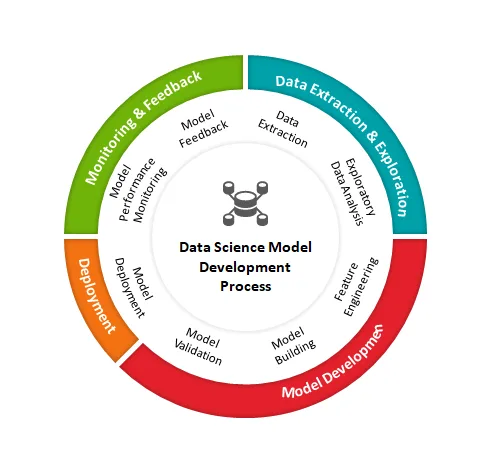
\includegraphics[scale=0.45]{figure/data-science-lifecycle.png}
\end{figure}

\end{frame}
%---------------------------------------------------------

\begin{frame}
\frametitle{Goals}
    \begin{itemize}
        \item Study the features of MLOps
        \item Study the different technologies to build an MLOps architecture
        \item Implement an MLOps architecture % to be used as template for future projects
    \end{itemize}
\end{frame}

%---------------------------------------------------------
%Example of the \pause command
\begin{frame}
\frametitle{Features}

\begin{columns}
\column{0.5\textwidth}
    \begin{itemize}
        \item Focus on the process
        \item Avoid handover between teams
        \item Reproducibility
        \item \textcolor{blue}{Experiment Tracking}
        \item Code Versioning and \\ \textcolor{blue}{Data Versioning}
        \item Modularity
    \end{itemize}

\column{0.5\textwidth}
    \begin{itemize} \pause
        \item Automation
        \item CI / CD
        \item \textcolor{blue}{Continuous Training}
        \item \textcolor{blue}{Continuous Monitoring}
        \item Testing + \\ \textcolor{blue}{Data and Models Validation}
        \item Monitoring
    \end{itemize}
\end{columns}

%In this slide \pause

%the text will be partially visible \pause

%And finally everything will be there
\end{frame}
%---------------------------------------------------------

%---------------------------------------------------------

\begin{frame}
\frametitle{The reference architecture}

\frametitle{The reference architecture}
\begin{figure}
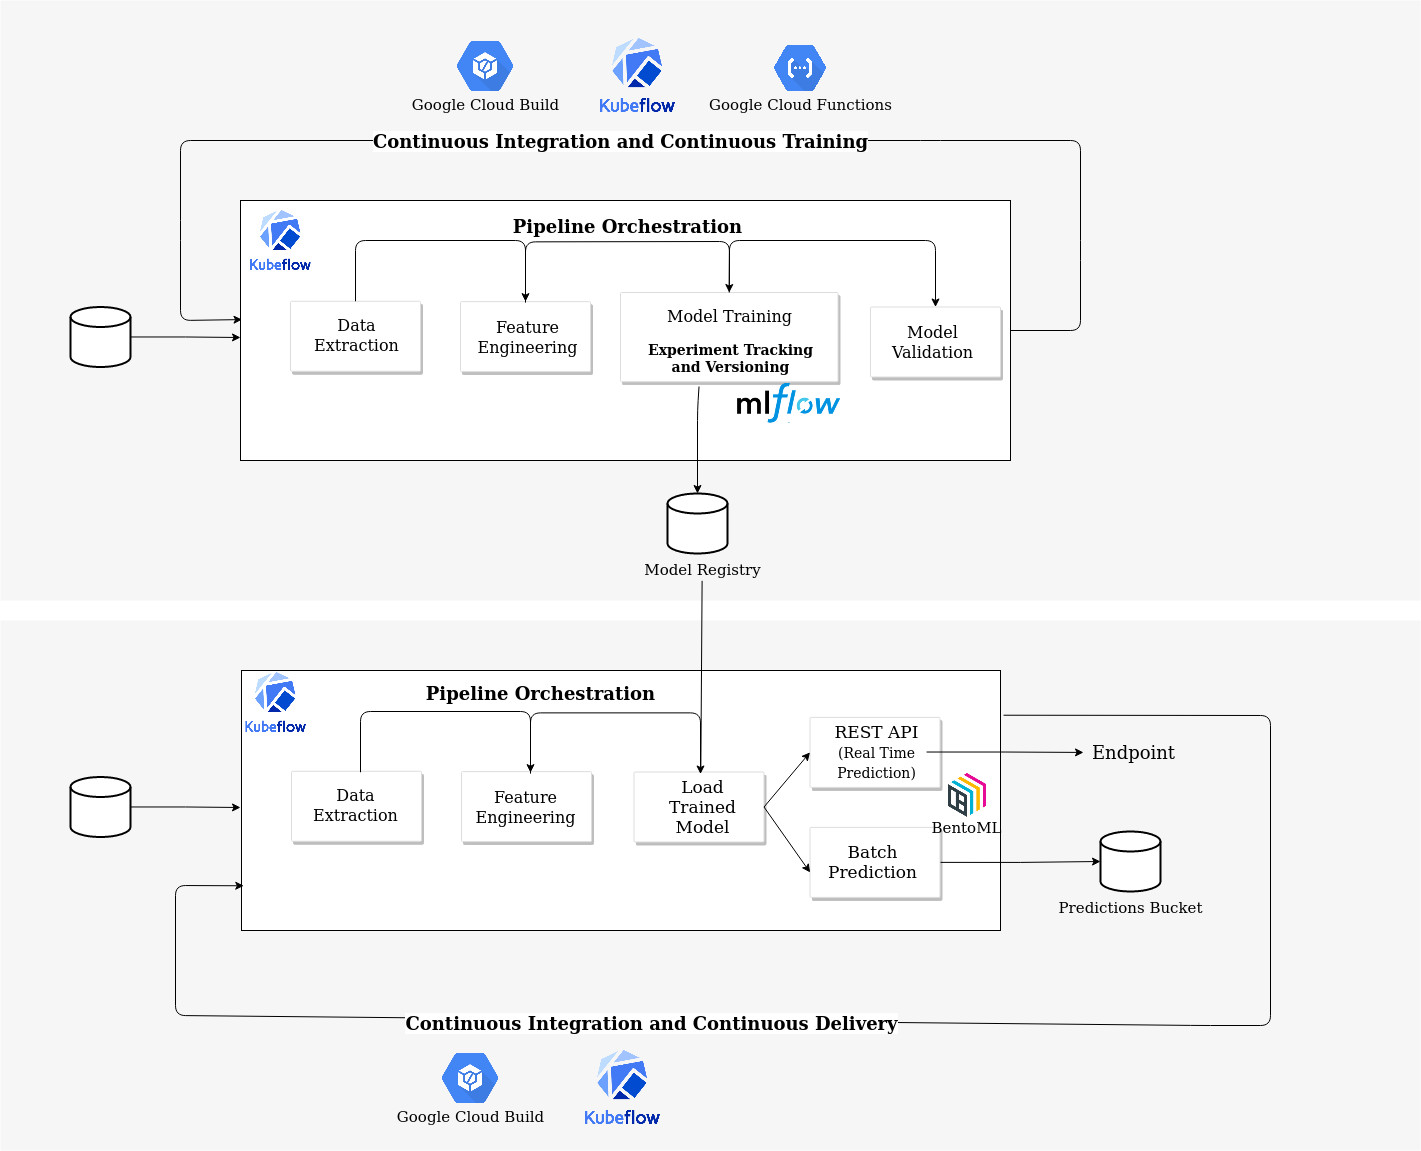
\includegraphics[scale=0.2]{figure/MLOps_Architecture_example.png}
\caption{The designed and implemented reference architecture}
\end{figure}

\end{frame}


\begin{frame}
\frametitle{The reference architecture}
\begin{figure}
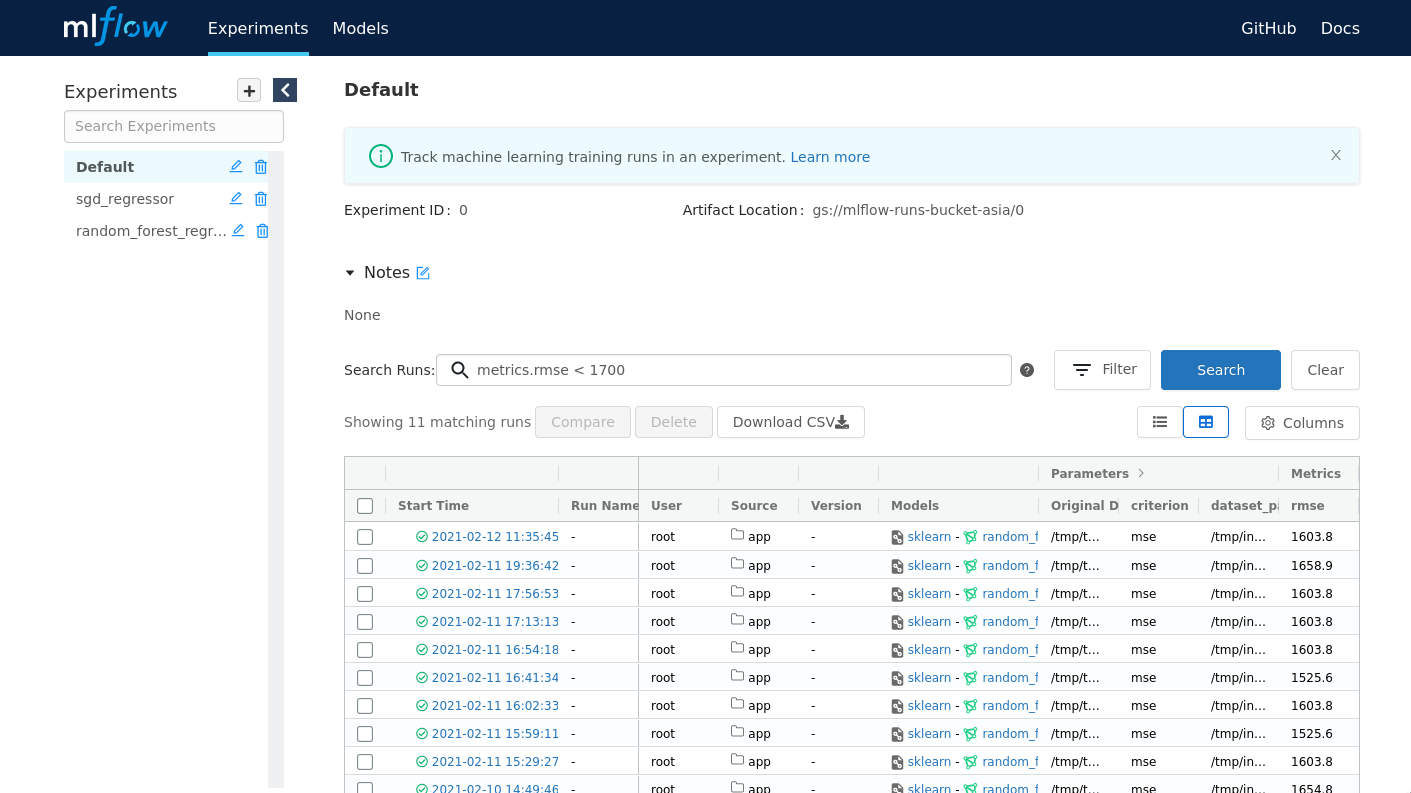
\includegraphics[scale=0.35]{figure/mlflow_filter_metrics.png}
\end{figure}

\end{frame}

\begin{frame}
\frametitle{The reference architecture}
\begin{figure}
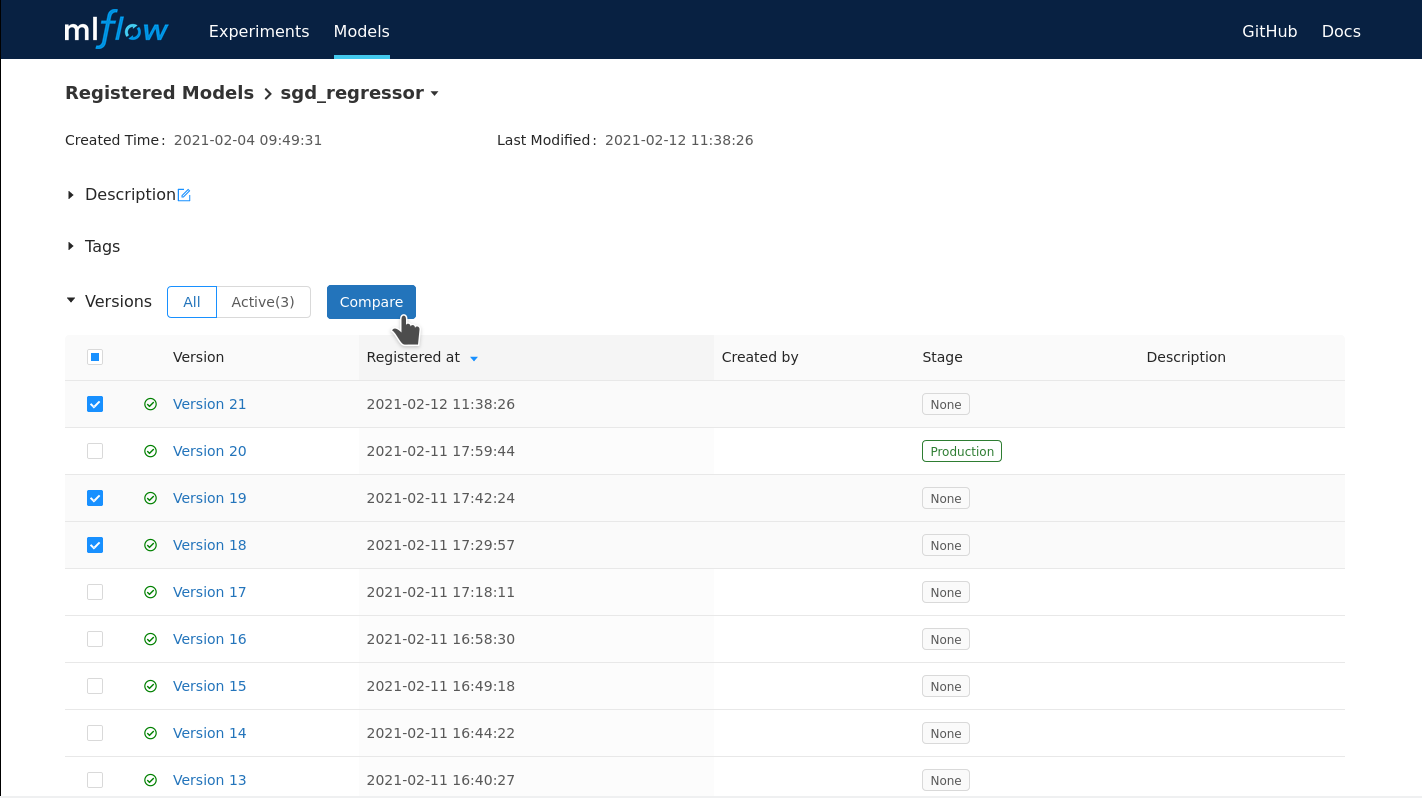
\includegraphics[scale=0.35]{figure/mlflow_model_versioning.png}
\end{figure}

\end{frame}

\begin{frame}
\frametitle{The reference architecture}
\begin{figure}
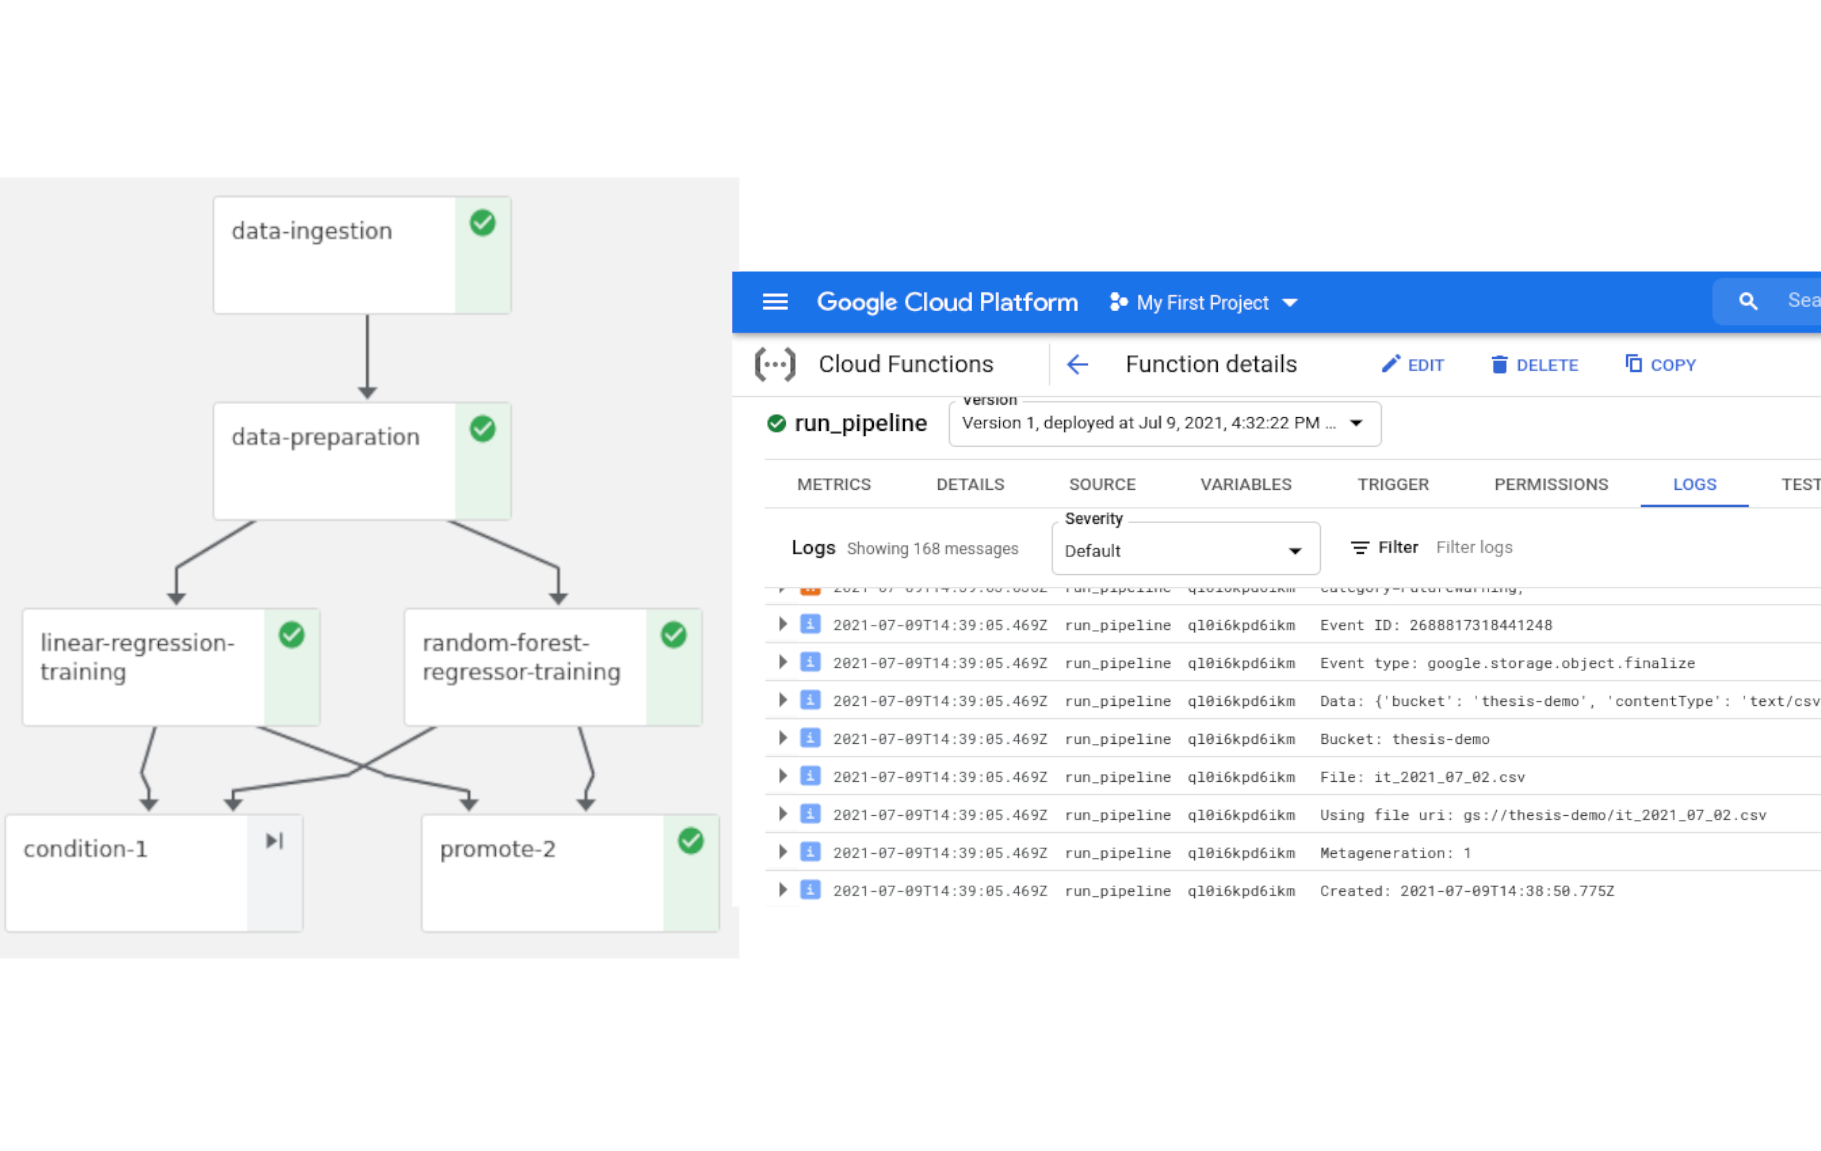
\includegraphics[scale=0.8]{figure/kubeflow_pipeline_gcf.png}
\end{figure}

\end{frame}

\begin{frame}
\frametitle{The reference architecture}
\begin{figure}
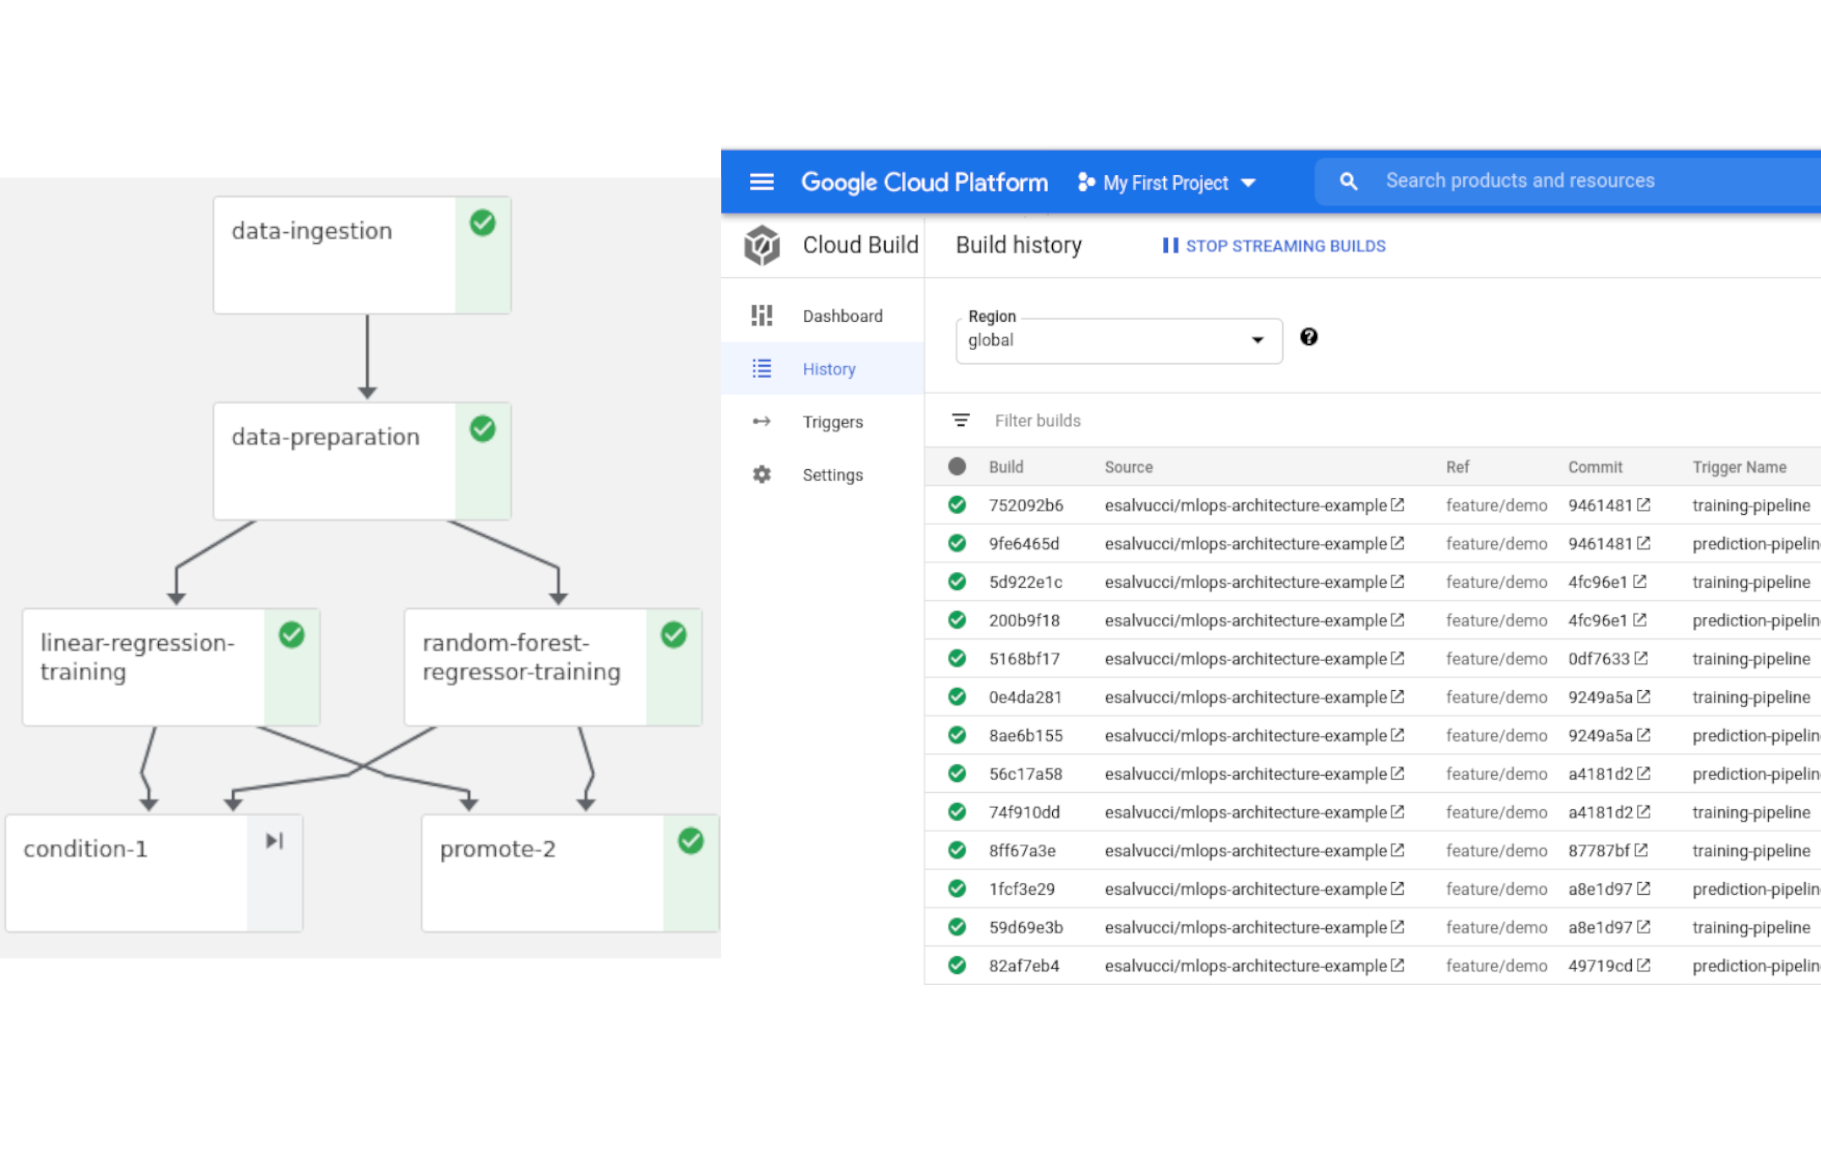
\includegraphics[scale=0.80]{figure/kubeflow_pipeline_gcb.png}
\end{figure}

\end{frame}

\begin{frame}
\frametitle{Use cases and scenarios}
\begin{figure}
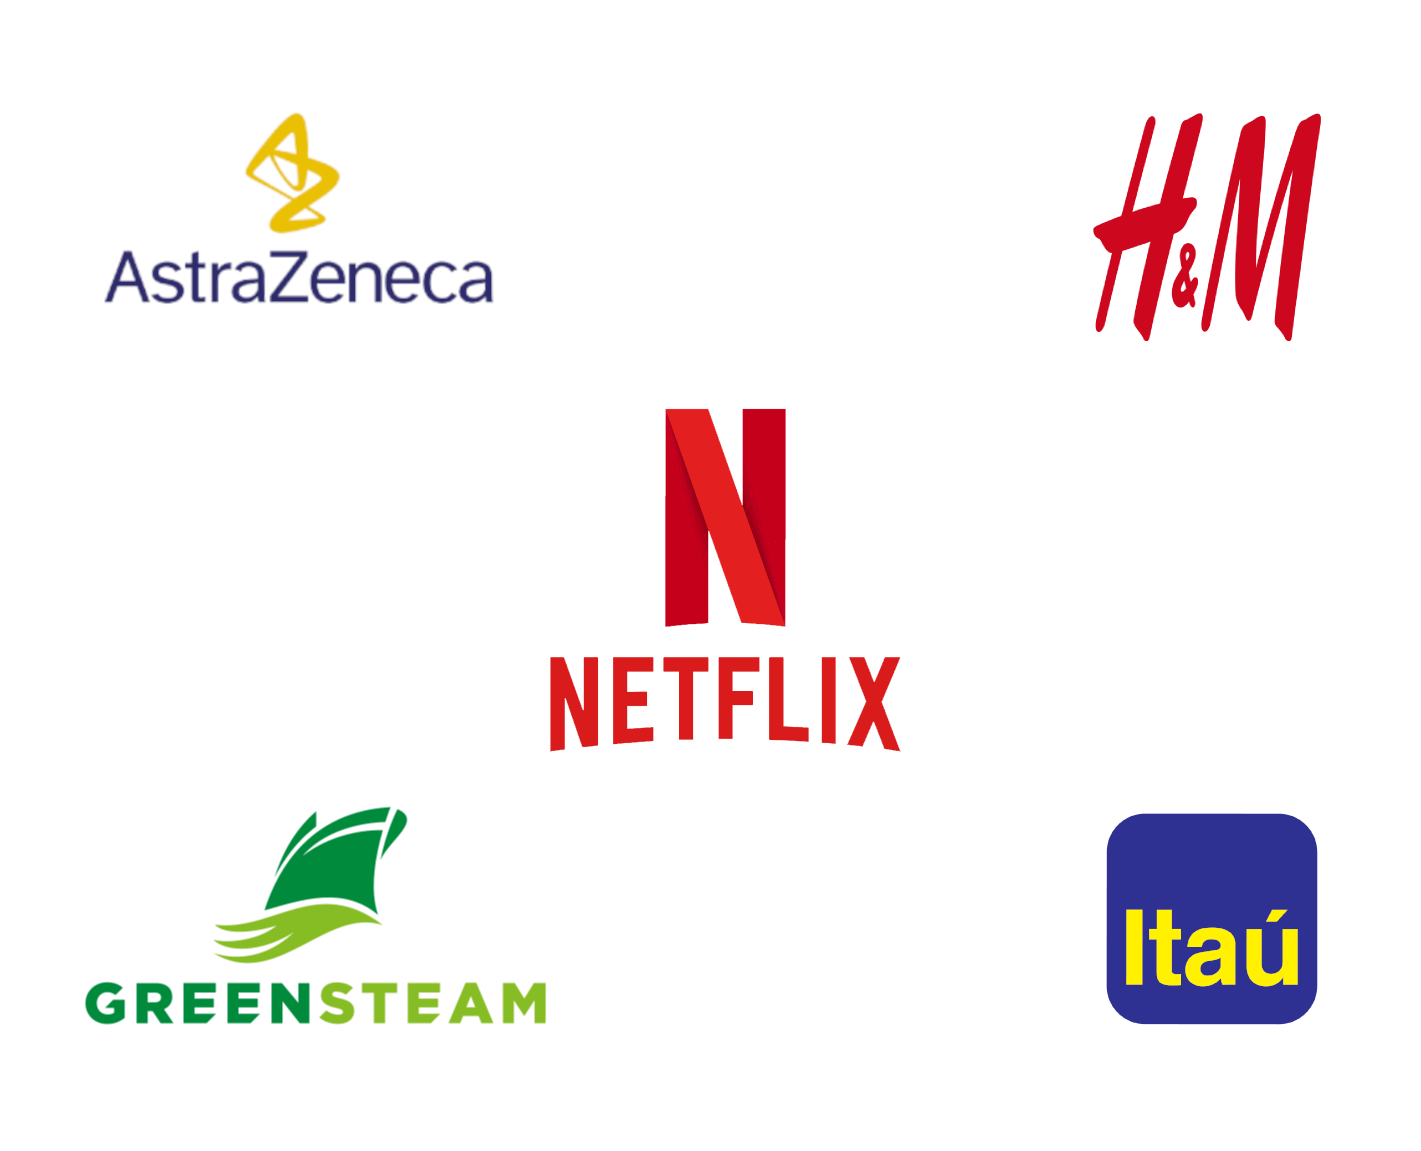
\includegraphics[scale=0.8]{figure/use_cases_companies.png}
\end{figure}
\end{frame}

%---------------------------------------------------------
%Two columns
\begin{frame}
\frametitle{Future works}

\begin{block}{The implemented architecture}
    \begin{itemize}
        \item Implement serving through Seldon Core
        \item Include Monitoring tools in the implemented architecture
    \end{itemize}
\end{block}

\end{frame}


\begin{frame}
\frametitle{Future works}

\begin{block}{MLOps} 
    \begin{itemize}
        \item MLOps tools are still immature and require to be improved
        \item ``\textit{MLOps market is expected to expand to nearly US\$4 billion by 2025}" (Cognilytica)
        \item MLOps will impact Machine Learning in the same way DevOps impacted software development
    \end{itemize}
\end{block}

\end{frame}
%---------------------------------------------------------

\section{A survey of technologies for MLOps}

%---------------------------------------------------------
%Highlighting text

\begin{frame}
\frametitle{MLOps}

\begin{figure}
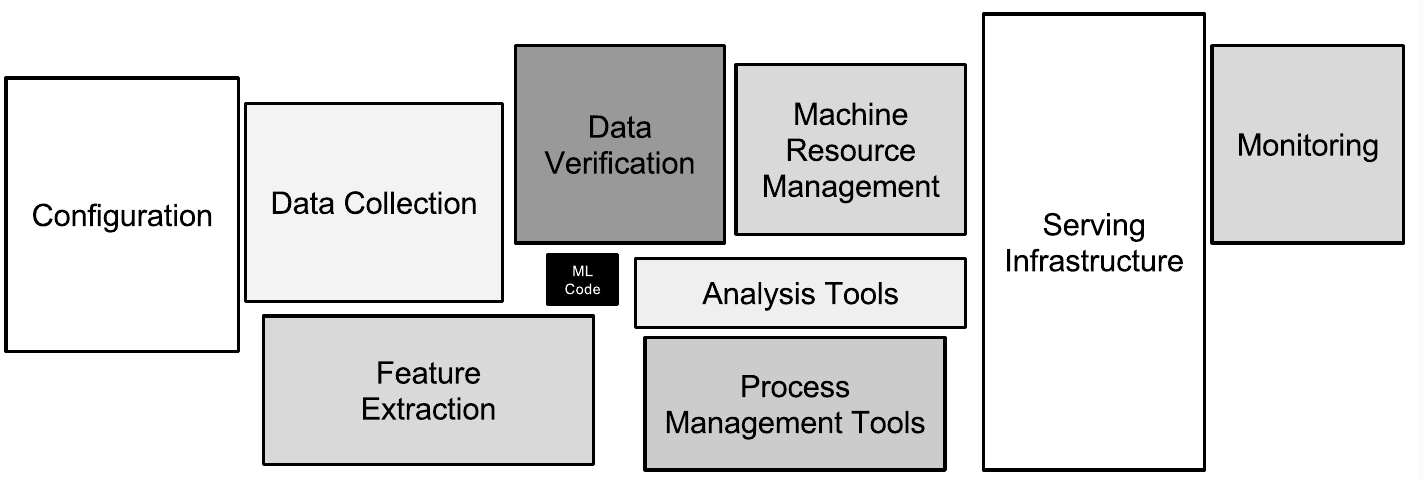
\includegraphics[scale=0.3]{figure/ml_small_fraction.png}
\end{figure}

\end{frame}


\begin{frame}
\frametitle{A survey of technologies for MLOps}

\begin{block}{Experiment Tracking}
    \begin{itemize}
        \item MLFlow
        \item DVC
    \end{itemize}
\end{block}

\end{frame}

\begin{frame}
\frametitle{A survey of technologies for MLOps}

\begin{block}{Pipeline orchestration}
    \begin{itemize}
        \item Kubeflow
        \item Airflow
        \item DVC
    \end{itemize}
\end{block}

\end{frame}

\begin{frame}
\frametitle{A survey of technologies for MLOps}

\begin{block}{Serving}
    \begin{itemize}
        \item Seldon Core
        \item KFServing
        \item BentoML
    \end{itemize}
\end{block}

\end{frame}

\begin{frame}
\frametitle{The reference architecture}
\begin{figure}
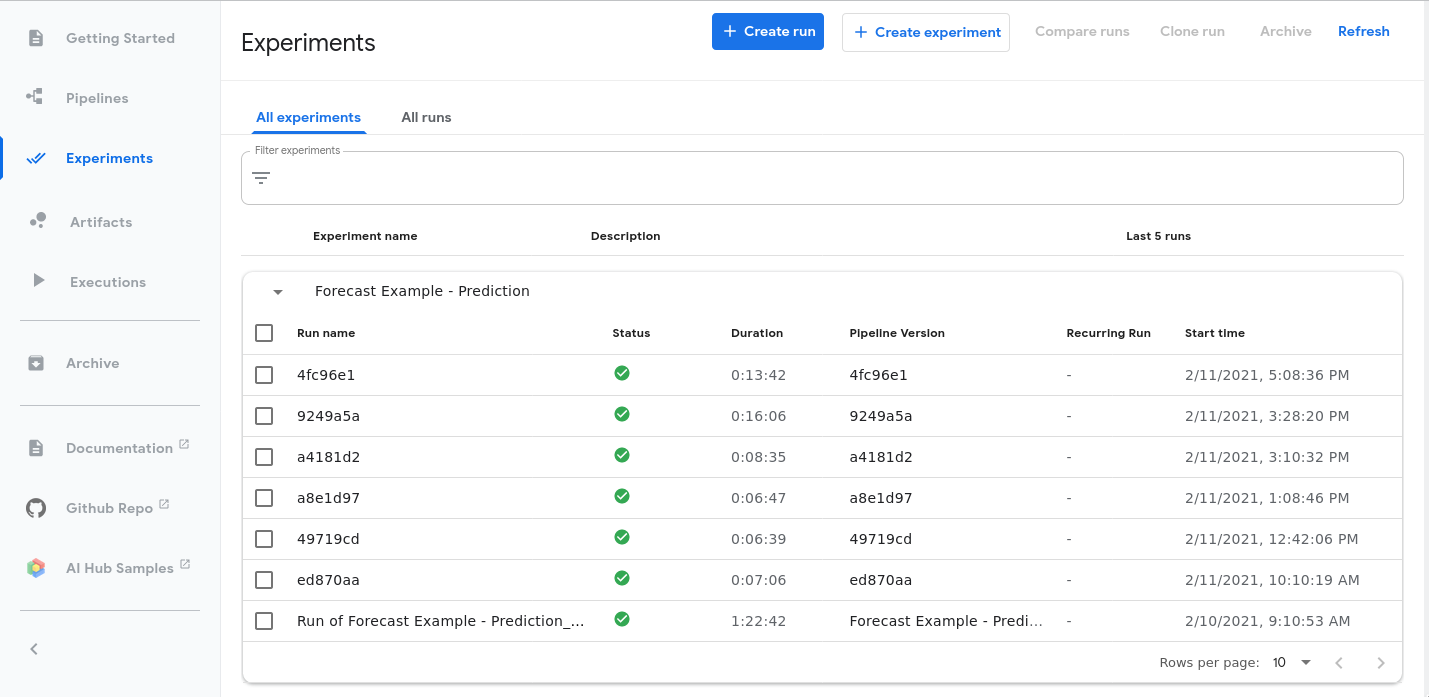
\includegraphics[scale=0.40]{figure/kubeflow_prediction_pipeline.png}
\end{figure}

\end{frame}

\end{document}

%In this slide, some important text will be
%\alert{highlighted} because it's important.
%Please, don't abuse it.


%\begin{alertblock}{Important theorem}
%Sample text in red box
%\end{alertblock}

%\begin{examples}
%Sample text in green box. The title of the block is ``Examples".
%\end{examples}
